%   Simulators for testing
%       + SITL, JSBSim, Flightgear, Simple GNSS
\subsection{Vehicle}
    \paragraph{JSBsim}
        %http://jsbsim.sourceforge.net/
        %http://wiki.flightgear.org/JSBSim
        %Bare bones system model that runs on multiple OS's
        %"Flight dynamics model"
    
    \paragraph{Flightgear}
        %http://wiki.flightgear.org/Flightgear
        %Built on top of jsbsim. Adds a visual interface, cross platform
        %Flight simulator 
    
\subsection{GNSS}
    %Delay introduced. EKF get's externalEstimatedState at the same time as the simulator. GNSS-message arrives at the next iteration
    %Pseudorange and doppler
    %Constellation of six stationary satellites with no noise or bias
    %Subscribes to ExternalStateEstimate
    
    A simple simulator of a stationary satellite was implemented in DUNE. Several tasks of the simulator where then called, each representing a unique satellite. The satellites were initialized with respect to latitude, longitude and elevation, as it is then far easier to set valid coordinates with respect to an observer than with the ECEF frame of reference.\\

    To find satellite coordinates that were reasonably close to the real world, a live updated satellite map was used, and coordinates translated to the \textit{llh} format.

    %Simulator description/Problems
    The simulator calculates the range between vehicle and satellite and adds Gaussian noise.\\ 

    \todo{rewrite. Needs header sentence}
    The input to the simulator is an IMC message containing the true state of the system, received at a frequency of 10 Hz. This is close to the frequency one might expect to receive actual GNSS measurements, and therefore, a GNSS IMC message is output for every incoming true state. However, as all the satellites in the constellation are run as separate tasks, the true state will be received at the same time for all satellites. As a result, GNSS-messages will be dispatched approximately simultaneously, resulting in messages being sent in \textit{bursts}. This leads to two problems; The timestep between messages in one burst might be excessively small, yet on the other hand, the time step between bursts may well be too large\todo{Bad statement? Not too large?}. This can lead to significant estimation errors and instability \todo{cite}. By introducing distinct delays to each of the satellites, the dispatch of GNSS messages are spread out evenly. Another option would buffer the GNSS messages at the MEKF and input all of the data together \todo{Superposition/separation principle?}.
    \todo{forsinkelse i posisjon mellom simulator og filter (noen pseudoranges blir feil/utdatert)}

\subsection{ArduPilot Software In The Loop}
    %http://ardupilot.github.io/MAVProxy/html/index.html
    %Neptus, mavproxy, flightgear, gnss / rtklib playback file
\begin{figure}
    \centering
    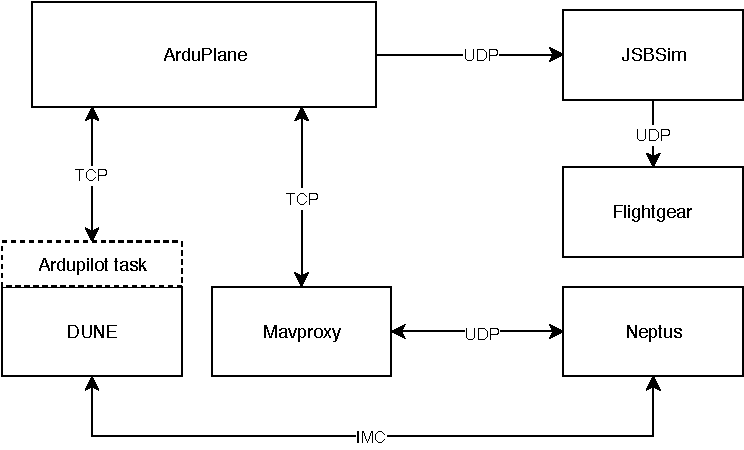
\includegraphics{Images/Simulator.pdf}
    \caption{Simulator block diagram}
    \label{fig:sim-diag}
\end{figure}
%\includepdf[pages=-]{Images/sim_diagram.pdf}
%\includepdf{Images/sim_diagram.pdf}
%SIM_VEHICLE: "mavproxy.py" "--master" "tcp:127.0.0.1:5760" "--sitl" "127.0.0.1:5501" "--out" "127.0.0.1:14550" "--out" "127.0.0.1:14551" "--map" "--console"
%flightgear: 5503
%ntnu-x8-001 on AP serial 2
%dune task: tcp:5760

%Initialization
\todo{Playback test}